\documentclass[12pt,UTF8,fleqn]{ctexart}
\usepackage{ctex,amsmath,amssymb,geometry,fancyhdr,bm,amsfonts,mathtools,extarrows,graphicx,url,enumerate,xcolor,float,multicol,wasysym}
\usepackage{subfigure}

\allowdisplaybreaks[4]
% 加入中文支持
\newcommand\Set[2]{\left\{#1\ \middle\vert\ #2 \right\}}
\newcommand\Lim[0]{\lim\limits_{n\rightarrow\infty}}
\newcommand\LIM[2]{\lim\limits_{#1\rightarrow#2}}
\newcommand\Ser[1]{\sum_{n=#1}^\infty}
\newcommand{\SER}[2]{\sum_{#1=#2}^\infty}
\newcommand{\Int}[4]{\varint\nolimits_{#1}^{#2}#3\mathrm d#4}
\newcommand{\aIInt}[1]{\iint\limits_{#1}}
\newcommand{\IInt}[3]{\iint\limits_{#1}#2\mathrm d#3}
\newcommand{\varIInt}[4]{\iint\limits_{#1}#2\mathrm d#3\mathrm d#4}
\newcommand{\IIInt}[3]{\iiint\limits_{#1}#2\mathrm d#3}
\newcommand{\varIIInt}[5]{\iiint\limits_{#1}#2\mathrm d#3\mathrm d#4\mathrm d#5}
\newcommand{\LInt}[3]{\varint\nolimits_{#1}#2\mathrm d#3}
\newcommand{\LOInt}[3]{\varoint\nolimits_{#1}#2\mathrm d#3}
\newcommand{\LLInt}[4]{\varint\nolimits_{#1}\nolimits^{#2}#3\mathrm d#4}
\newcommand{\BLInt}[2]{\varint\nolimits_{#1}#2}
\newcommand{\varBLInt}[3]{\varint\nolimits_{#1}\nolimits^{#2}#3}
\newcommand{\BLOInt}[2]{\varoint\nolimits_{#1}#2}
\newcommand{\SIInt}[3]{\iint\limits_{#1}#2\mathrm d#3}
\newcommand{\md}[1]{\mathrm d#1}
\newcommand{\BSIInt}[2]{\iint\limits_{#1}#2}
\newcommand{\pp}[2]{\frac{\partial #1}{\partial #2}}
\newcommand{\BSOIInt}[2]{\oiint\nolimits_{#1}#2}
\geometry{a4paper,scale=0.80}
\pagestyle{fancy}
\rhead{习题13.4}
\lhead{基础习题课讲义}
\chead{微积分B(2)}
\begin{document}
\setcounter{section}{22}
\section{第二型曲面积分}
\subsection{知识结构}
\noindent第13章向量场的微积分
	\begin{enumerate}
		\item[13.4]向量场的曲面积分
			\begin{enumerate}
				\item[13.4.1]有向曲面
				\item[13.4.2]向量场曲面积分的概念和计算
			\end{enumerate}
	\end{enumerate}
\subsection{第二型曲面积分的计算}
第二型曲面积分$\BSIInt S{\bm F\bm\cdot\md\bm S}$中:
\setlength{\mathindent}{1cm}
\[\bm F(x,y,z)=(X(x,y,z),Y(x,y,z),Z(x,y,z))\in C(S),\text{为空间向量场;}\]
\[\begin{aligned}
\md\bm S=\bm n\md S=(\cos\alpha,\cos\beta,\cos\gamma)\md S&=(\cos\alpha\md S,\cos\beta\md S,\cos\gamma\md S)\\&=(\md y\wedge\md z,\md z\wedge\md x,\md x\wedge\md y),\text{为有向面积元素;}
\end{aligned}\]

\noindent有向曲面$S$可有以下几种形式:
\begin{enumerate}
\item显示方程
\begin{enumerate}
\item$S:z=f(x,y),(x,y)\in D_{xy}$. 此时
\setlength{\mathindent}{0cm}
\[\bm n=\pm(-\pp fx,-\pp fy,1)\frac1{\sqrt{(\pp fx)^2+(\pp fy)^2+1}},\ \md S=\sqrt{(\pp fx)^2+(\pp fy)^2+1}\md x\md y\]
\[\md\bm S=\bm n\md S=\pm(-\pp fx,-\pp fy,1)\md x\md y=(\md y\wedge\md z,\md z\wedge\md x,\md x\wedge\md y).\]
若在曲面$S$的$+z$侧做积分取$+$号,若在曲面$S$的$-z$侧做积分取$-$号.
\setlength{\mathindent}{0cm}
\[\begin{aligned}
\text{故}&\BSIInt S{\bm F\bm\cdot\md\bm S}\\
=&\BSIInt S{X(x,y,z)\md y\wedge\md z+Y(x,y,z)\md z\wedge\md x+Z(x,y,z)\md x\wedge\md y}\\
=&\pm\BSIInt S{[-X(x,y,f(x,y))\pp fx-Y(x,y,f(x,y))\pp fy+Z(x,y,f(x,y))]\md x\md y}
\end{aligned}\]
【利用该公式进行计算的习题:8.(第三类题目)】

注意此时$\md x\wedge\md y=\pm\md x\md y$,在曲面$+z$侧积分,取$+$号,在曲面$-z$侧积分,取$-$号.

【利用这一点进行计算的习题:1,2,3,4,5.(第一类题目) 7,10.(第二类题目)】
\item$S:x=g(y,z),(y,x)\in D_{yz}$. 可进行类似的推导.

注意此时$\md y\wedge\md z=\pm\md y\md z$,在曲面$+x$侧积分,取$+$号,在曲面$-x$侧积分,取$-$号.
\item$S:y=g(z,x),(z,x)\in D_{zx}$. 可进行类似的推导.

注意此时$\md z\wedge\md x=\pm\md z\md x$,在曲面$+y$侧积分,取$+$号,在曲面$-y$侧积分,取$-$号.
\end{enumerate}
\item参数方程
\begin{enumerate}
\item[]$S:\begin{cases}
x=x(u,v),\\
y=y(u,v),\\
z=z(u,v),
\end{cases}(u,v)\in D_{uv}$. 此时
\setlength{\mathindent}{0cm}
\[\bm n=\pm(A,B,C)\frac1{\sqrt{A^2+B^2+C^2}},\ \md S=\sqrt{A^2+B^2+C^2}\md u\md v,\]
\[\md\bm S=\bm n\md S='\pm'(A,B,C)\md S=(\md y\wedge\md z,\md z\wedge\md x,\md x\wedge\md y),\]
\[\text{其中}A=\frac{\mathrm D(y,z)}{\mathrm D(u,v)},\ B=\frac{\mathrm D(z,x)}{\mathrm D(u,v)},\ C=\frac{\mathrm D(x,y)}{\mathrm D(u,v)}.\]
若在曲面的$+x$侧积分,则选取$\pm$号使得$\pm A>0$;若在曲面的下侧积分,则选取$\pm$号使得$\pm A<0$;若在曲面的$+y$侧积分,则选取$\pm$号使得$\pm B>0$;若在曲面的$-y$侧积分,则选取$\pm$号使得$\pm B<0$;若在曲面的$+z$侧积分,则选取$\pm$号使得$\pm C>0$;若在曲面的$-z$侧积分,则选取$\pm$号使得$\pm C<0$.
\setlength{\mathindent}{0cm}
\[\begin{aligned}
\text{故}&\BSIInt S{\bm F\bm\cdot\md\bm S}\\
=&\BSIInt S{X(x,y,z)\md y\wedge\md z+Y(x,y,z)\md z\wedge\md x+Z(x,y,z)\md x\wedge\md y}\\
=&\pm\BSIInt S{[X(x(u,v),y(u,v),z(u,v))A+YB+ZC]\md u\md v}.
\end{aligned}\]
【利用该公式进行计算的习题:9,6.(第五类题目)】

【其他类型的习题:9,11,6.(第四类题目)】
\end{enumerate}
\end{enumerate}
\subsection{习题13.4解答}
\noindent计算下列第二型曲面积分:
\begin{enumerate}
\item$\BSIInt S{(x^2+y^2)\md x\wedge\md y},S$为$x^2+y^2\leqslant1,z=0$的下侧.

解:$\BSIInt S{(x^2+y^2)\md x\wedge\md y}=\BSIInt{x^2+y^2\leqslant1}{(x^2+y^2)(-\md x\md y)}=-\Int0{2\pi}{}\theta\Int01{r^2\cdot r}r=-2\pi\cdot\frac14r^4\big|_0^1\\
=-\frac\pi2$.

\item$\BSIInt S{z\md x\wedge\md y},S$为$x^2+y^2+z^2=R^2$上半部分的下侧.

解:$\BSIInt S{z\md x\wedge\md y}=\BSIInt{x^2+y^2\leqslant R^2}{\sqrt{R^2-x^2-y^2}(-\md x\md y)}=-\Int0{2\pi}{}\theta\Int0R{\sqrt{R^2-r^2}\cdot r}r\\
=-2\pi(-\frac12)\frac1{1+\frac12}(R^2-r^2)^{\frac12+1}\big|_0^R=-\frac23\pi R^3$.

\item$\BSIInt S{xz^2\md x\wedge\md y},S$为$x^2+y^2+z^2=1$第一卦限部分的外侧.

\begin{figure}[H]
\begin{center}
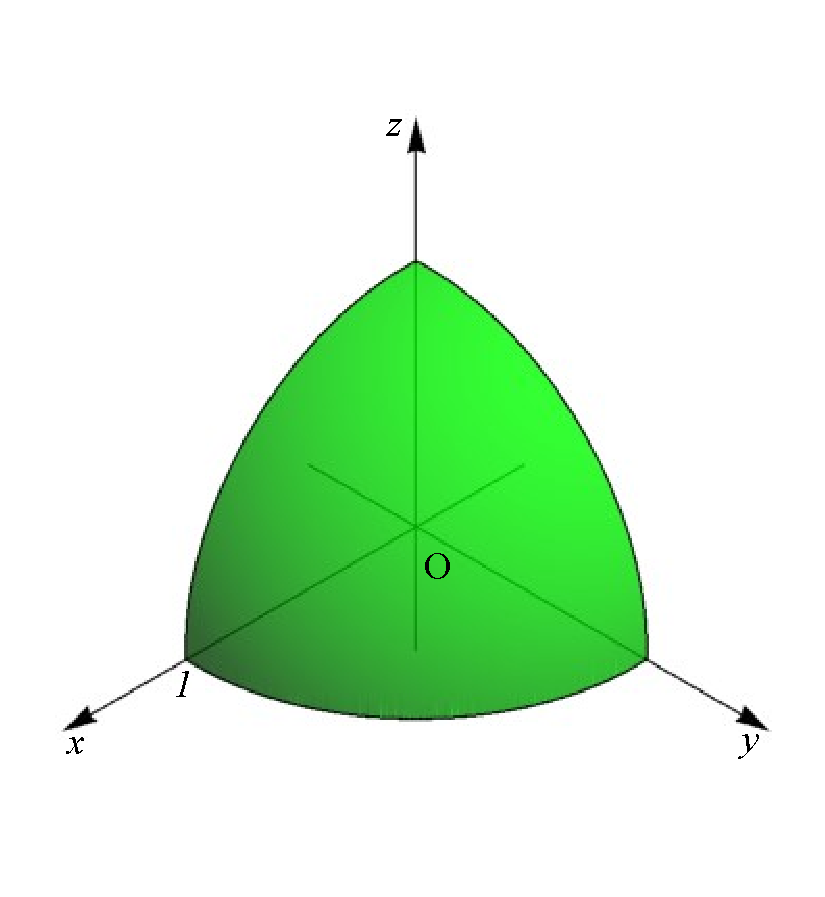
\includegraphics[height=0.5\textheight]{Figures23/Fig13-4-3.pdf}
\end{center}
\caption{习题13.4 3.题图示}
\label{13-4-3}
\end{figure}

解:曲面$S$的方程可以表示为$z=\sqrt{1-x^2-y^2},x^2+y^2\leqslant1,x\geqslant0,y\geqslant0$,

$\therefore\BSIInt S{xz^2\md x\wedge\md y}=\BSIInt{\substack{x^2+y^2\leqslant1,\\ x\geqslant0,y\geqslant0}}{x(1-x^2-y^2)\md x\md y}=\Int0{\frac\pi2}{}\theta\Int01{r\cos\theta(1-r^2)\cdot r}r\\
=\Int0{\frac\pi2}{\cos\theta}\theta\Int01{r^2(1-r^2)}r=1\cdot(\frac13r^2-\frac15r^5)\big|_0^1=\frac2{15}$.

\item$\BSIInt S{z^2\md x\wedge\md y},S$为$z=\sqrt{a^2-x^2-y^2}(a>0)$被圆柱面$x^2+y^2=ax$所截部分的上侧.

\begin{figure}[H]
\begin{center}
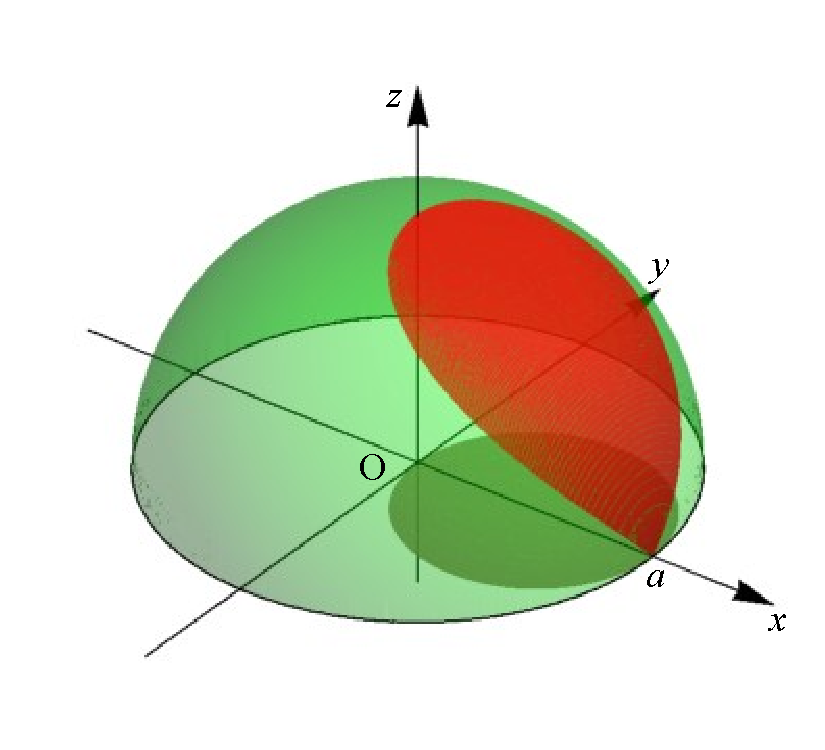
\includegraphics[height=0.5\textheight]{Figures23/Fig13-4-4.pdf}
\end{center}
\caption{习题13.4 4.题图示}
\label{13-4-4}
\end{figure}

解:$\BSIInt S{z^2\md x\wedge\md y}=\BSIInt{x^2+y^2\leqslant ax}{(a^2-x^2-y^2)\md x\md y}=\Int{-\frac\pi2}{\frac\pi2}{}\theta\Int0{a\cos\theta}{(a^2-r^2)\cdot r}r\\
=\Int{-\frac\pi2}{\frac\pi2}{(\frac12a^2r^2-\frac14r^4)\big|_0^{a\cos\theta}}\theta=\Int{-\frac\pi2}{\frac\pi2}{(\frac12a^4\cos^2\theta-\frac14a^4\cos^4\theta)}\theta=2\Int0{\frac\pi2}{(\frac12a^4\cos^2\theta-\frac14a^4\cos^4\theta)}\theta\\
=2(\frac12a^4\frac12\cdot\frac\pi2-\frac14a^4\frac34\cdot\frac12\cdot\frac\pi2)=\frac5{32}\pi a^4$.

\item$\BSIInt S{2y\md z\wedge\md x}$,其中$S$为锥面$y=\sqrt{x^2+z^2}$介于$y=1$和$y=2$之间的部分外侧.

\begin{figure}[H]
\begin{center}
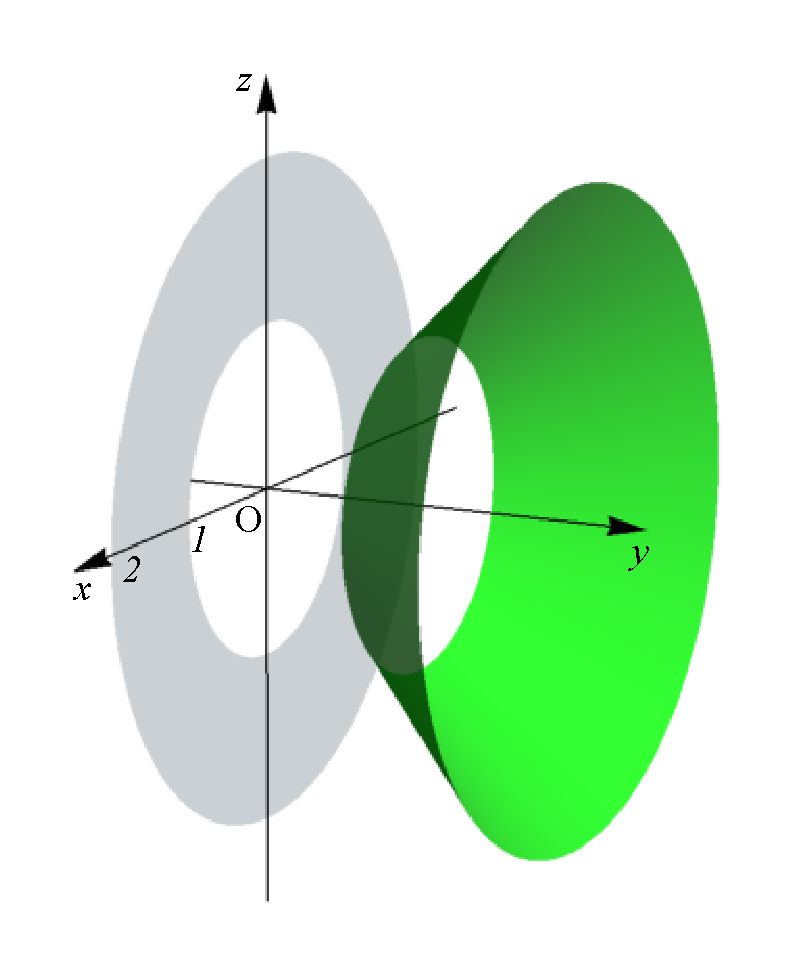
\includegraphics[height=0.5\textheight]{Figures23/Fig13-4-5.pdf}
\end{center}
\caption{习题13.4 5.题图示}
\label{13-4-5}
\end{figure}

解:$\BSIInt S{2y\md z\wedge\md x}=\BSIInt{1\leqslant x^2+z^2\leqslant4}{2\sqrt{x^2+z^2}(-\md x\md z)}=-\Int0{2\pi}{}\theta\Int12{2r\cdot r}r=-2\pi\frac23r^3\big|_1^2\\
=-\frac{28}3\pi$.

\item$\BSIInt S{x\md y\wedge\md z+z\md x\wedge\md y},S$为$x^2+y^2=a^2$在第一卦限中介于$z=0,z=h(h>0)$之间的部分,外侧为正.

\begin{figure}[H]
\begin{center}
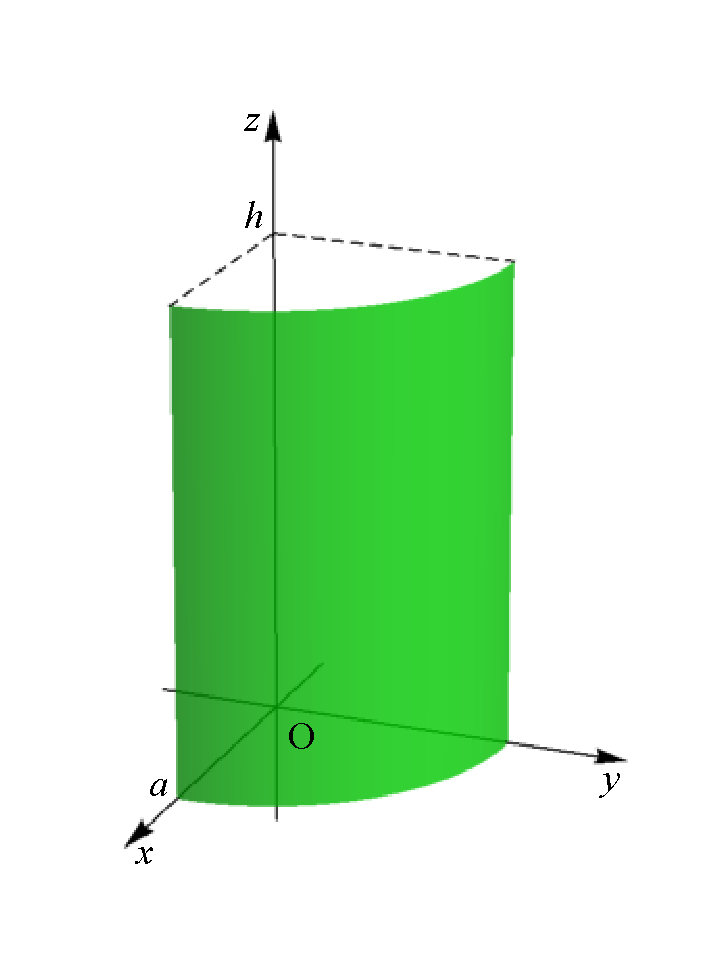
\includegraphics[height=0.5\textheight]{Figures23/Fig13-4-6.pdf}
\end{center}
\caption{习题13.4 6.题图示}
\label{13-4-6}
\end{figure}

解:方法1:令$\begin{cases}
x=a\cos\theta,\\
y=a\sin\theta,\\
z=z,
\end{cases}(\theta,z)\in D=\Set{(\theta,z)}{0\leqslant\theta\leqslant\frac\pi2,0\leqslant z\leqslant h}$,

则$A=\frac{\mathrm D(y,z)}{\mathrm D(\theta,z)}=\begin{vmatrix}
a\cos\theta&0\\
0&1
\end{vmatrix}=a\cos\theta,\ B=\frac{\mathrm D(z,x)}{\mathrm D(\theta,z)}=\begin{vmatrix}
0&1\\
-a\sin\theta&0
\end{vmatrix}=a\sin\theta,\\
C=\frac{\mathrm D(x,y)}{\mathrm D(\theta,z)}=\begin{vmatrix}
-a\sin\theta&0\\
a\cos\theta&0
\end{vmatrix}=0$,

$\therefore\md\bm S=(A,B,C)\md\theta\md z=(a\cos\theta,a\sin\theta,0)\md\theta\md z=(\md y\wedge\md z,\md z\wedge\md x,\md x\wedge\md y)$,

$\therefore\BSIInt S{x\md y\wedge\md z+z\md x\wedge\md y}=\BSIInt D{a\cos\theta\cdot a\cos\theta\md\theta\md z+z\cdot0}=a^2\Int0{\frac\pi2}{\cos^2\theta}\theta\Int0h{}z=\frac\pi4a^2h$.

方法2:曲面$S$的正向单位法向量可以表示为$\bm n=\frac1a(x,y,0)$,

$\therefore\md\bm S=\bm n\md S=\frac1a(x,y,0)\md S=(\md y\wedge\md z,\md z\wedge\md x,\md x\wedge\md y)$,

$\therefore\BSIInt S{x\md y\wedge\md z+z\md x\wedge\md y}=\BSIInt S{x\cdot\frac1ax\md S+z\cdot0}=\frac1a\BSIInt S{x^2\md S}$,

$\because$曲面$S$关于平面$y=x$对称,

$\therefore$上式$=\frac1a\frac12\BSIInt S{(x^2+y^2)\md S}=\frac1{2a}\BSIInt S{a^2\md S}=\frac{a^2}{2a}\BSIInt S{\md S}=\frac a2\cdot\frac14\cdot2\pi a\cdot h=\frac\pi4a^2h$.

\item$\BSIInt S{z\md x\wedge\md y+\md y\wedge\md z},S$为平面$x+y-z=1$在第五卦限中的部分下侧.

\begin{figure}[H]
\begin{center}
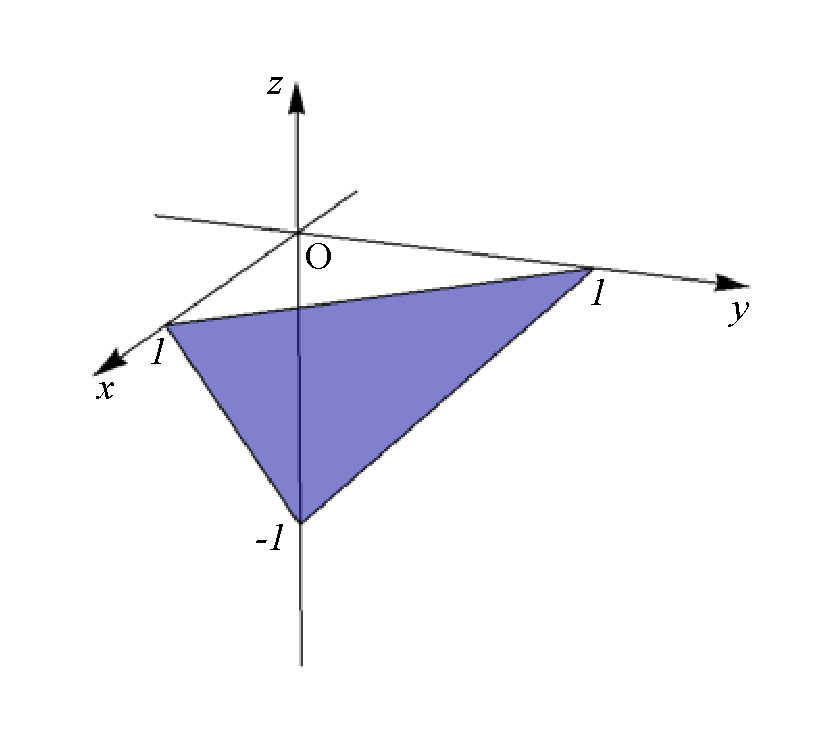
\includegraphics[height=0.5\textheight]{Figures23/Fig13-4-7.pdf}
\end{center}
\caption{习题13.4 7.题图示}
\label{13-4-7}
\end{figure}

解:方法1:$\BSIInt S{z\md x\wedge\md y+\md y\wedge\md z}=\BSIInt S{z\md x\wedge\md y}+\BSIInt S{\md y\wedge\md z}\\
=\BSIInt{D_{xy}}{(x+y-1)(-\md x\md y)}+\varIInt{D_{yz}}{}yz=\BSIInt{D_{xy}}{(1-x-y)\md x\md y}+\varIInt{D_{yz}}{}yz$,

其中$D_{xy}$与$D_{yz}$为$S$在$xOy$平面和$yOz$平面上的投影,$D_{xy}$关于$y=x$对称,

$\therefore$上式$=\varIInt{D_{xy}}{}xy-2\varIInt{D_{xy}}xxy+\varIInt{D_{yz}}{}yz=\frac12-2\Int01xx\Int0{1-x}{}y+\frac12\\
=1-2\Int01{x(1-x)}x=1-2(\frac12x^2-\frac13x^3)\big|_0^1=\frac23$.

方法2:平面$S$的方程可表示为$z=x+y-1,(x,y)\in D=\Set{(x,y)}{0\leqslant x\leqslant1,0\leqslant y\leqslant1-x}$,

$\therefore\md\bm S=-(-\pp zx,-\pp zy,1)\md x\md y=(1,1,-1)\md x\md y=(\md y\wedge\md z,\md z\wedge\md x,\md x\wedge\md y)$,

$\therefore\BSIInt S{z\md x\wedge\md y+\md y\wedge\md z}=\BSIInt D{[(x+y-1)(-\md x\md y)+\md x\md y]}=\varIInt D{(2-x-y)}xy$,

$\because$区域$D$关于$y=x$对称,

$\therefore$上式$=2\varIInt D{}xy-2\varIInt Dxxy=2\cdot\frac12-2\Int01xx\Int0{1-x}{}y=1-2\Int01{x(1-x)}x\\
=1-2(\frac12x^2-\frac13x^3)\big|_0^1=\frac23$.

%方法3:平面$S$的单位法向量为$\bm n=\frac1{\sqrt3}(1,1,-1)$,
%
%$\therefore\md\bm S=\bm n\md S=\frac1{\sqrt3}(1,1,-1)\md S=(\md y\wedge\md z,\md z\wedge\md x,\md x\wedge\md y)$,
%
%$\therefore\BSIInt S{z\md x\wedge\md y+\md y\wedge\md z}=\BSIInt S{-\frac z{\sqrt3}\md S+\frac1{\sqrt3}\md S}=\frac1{\sqrt3}\SIInt S{(1-z)}S$,
%
%平面$S$的方程可表示为$z=x+y-1,(x,y)\in D_{xy}=\Set{(x,y)}{0\leqslant x\leqslant1,0\leqslant y\leqslant1-x}$
%
%$\therefore$上式$=\frac1{\sqrt3}\varIInt{D_{xy}}{[1-(x+y-1)]\sqrt{(\pp zx)^2+(\pp zy)^2+1^2}}xy\\
%=\frac1{\sqrt3}\varIInt{D_{xy}}{[1-(x+y-1)]\sqrt{1^2+1^2+1^2}}xy=\varIInt{D_{xy}}{(2-x-y)}xy$,\\
%$\because D_{xy}$关于$y=x$对称,
%
%$\therefore$上式$=2\varIInt{D_{xy}}{}xy-2\varIInt{D_{xy}}{x}xy=2\cdot\frac12-2\Int01xx\Int0{1-x}{}y=1-2\Int01{x(1-x)}x\\
%=1-2(\frac12x^2-\frac13x^3)\big|_0^1=\frac23$.

\item$\BSIInt S{(y-z)\md y\wedge\md z+(z-x)\md z\wedge\md x+(x-y)\md x\wedge\md y},S$为$y=\sqrt{x^2+z^2},y=h(h>0)$所围区域的表面外侧.

\begin{figure}[H]
\begin{center}
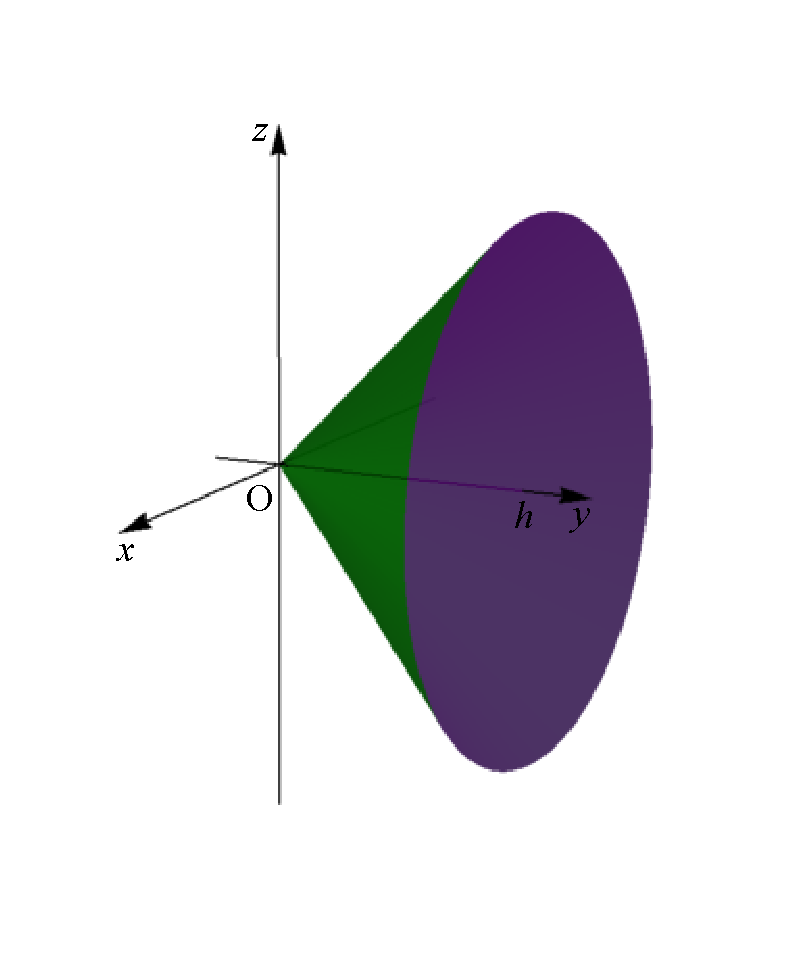
\includegraphics[height=0.5\textheight]{Figures23/Fig13-4-8.pdf}
\end{center}
\caption{习题13.4 8.题图示}
\label{13-4-8}
\end{figure}

解:$S$由锥面$S_1:y=\sqrt{x^2+z^2},x^2+y^2\leqslant h^2$的左侧和平面$S_2:y=h,x^2+y^2\leqslant h^2$的右侧组成,

在锥面$S_1$的左侧$\md\bm S=-(-\pp yx,1,-\pp yz)\md z\md x=(\frac x{\sqrt{x^2+z^2}},-1,\frac z{\sqrt{x^2+z^2}})\md z\md x\\
=(\md y\wedge\md z,\md z\wedge\md x,\md x\wedge\md y)$,

$\therefore\BSIInt{S_1}{(y-z)\md y\wedge\md z+(z-x)\md z\wedge\md x+(x-y)\md x\wedge\md y}\\
=\BSIInt{x^2+z^2\leqslant h^2}{(\sqrt{x^2+z^2}-z)\frac x{\sqrt{x^2+z^2}}\md z\md x-(z-x)\md z\md x+(x-\sqrt{x^2+z^2})\frac z{\sqrt{x^2+z^2}}\md z\md x}\\
=\varIInt{x^2+z^2\leqslant h^2}{(2x-2z)}zx$,

由对称性可知上式$=0$,

在平面$S_2$的右侧$\md\bm S=(-\pp yx,1,-\pp yz)\md z\md x=(0,1,0)\md z\md x=(\md y\wedge\md z,\md z\wedge\md x,\md x\wedge\md y)$,

$\therefore\BSIInt{S_2}{(y-z)\md y\wedge\md z+(z-x)\md z\wedge\md x+(x-y)\md x\wedge\md y}=\varIInt{x^2+z^2\leqslant h^2}{0+(z-x)+0}zx$,

由对称性可知上式$=0$,

$\therefore\BSIInt S{(y-z)\md y\wedge\md z+(z-x)\md z\wedge\md x+(x-y)\md x\wedge\md y}\\
=(\BSIInt{S_1}+\BSIInt{S_2}{)(y-z)\md y\wedge\md z+(z-x)\md z\wedge\md x+(x-y)\md x\wedge\md y}\\
=0+0=0$.

\item$\BSOIInt S{x\md y\wedge\md z+y\md z\wedge\md x+z\md x\wedge\md y},S$为$x^2+y^2+z^2=R^2$的外侧.

解:球面$S$的外向单位法向量为$\bm n=\frac1R(x,y,z)$,

$\therefore\md\bm S=\frac1R(x,y,z)\md S$,

$\therefore\BSOIInt S{x\md y\wedge\md z+y\md z\wedge\md x+z\md x\wedge\md y}=\BSOIInt S{(x\cdot\frac xR+y\cdot\frac yR+z\cdot\frac zR)\md S}=\BSOIInt S{\frac{x^2+y^2+z^2}R\md S}\\
=R\BSOIInt S\md S=4\pi R^3$.

\item$\BSOIInt S{yz\md y\wedge\md z+zx\md z\wedge\md x+xy\md x\wedge\md y},S$为区域$\begin{cases}
x+y+z\leqslant a,a>0\\
x\geqslant0,y\geqslant0,z\geqslant0
\end{cases}$表面的外侧.

\begin{figure}[H]
\begin{center}
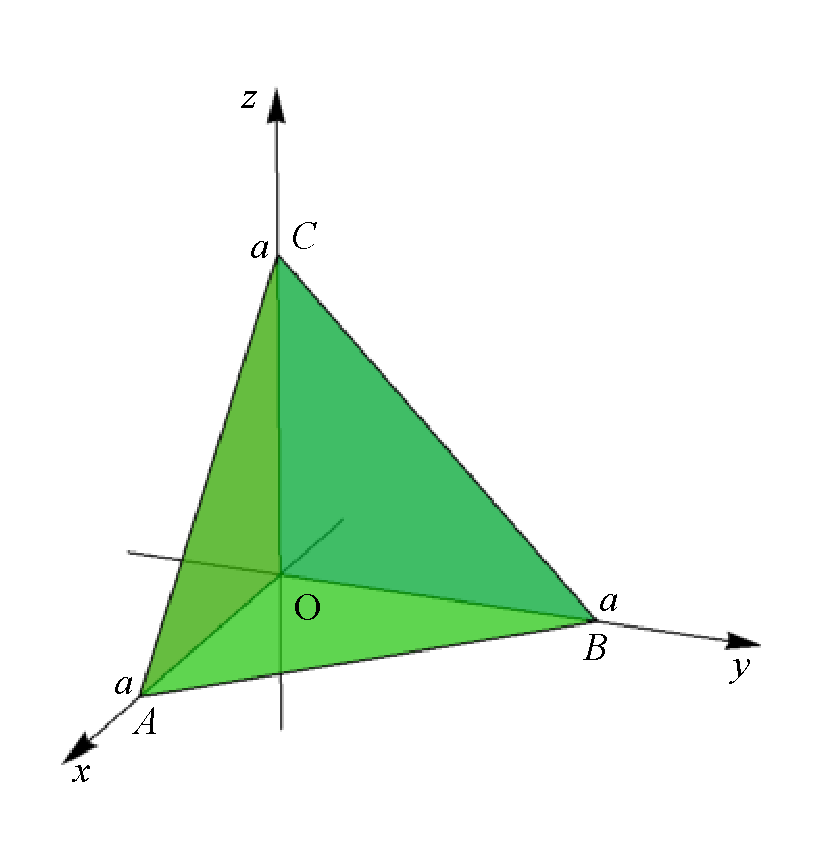
\includegraphics[height=0.7\textheight]{Figures23/Fig13-4-10.pdf}
\end{center}
\caption{习题13.4 10.题图示}
\label{13-4-10}
\end{figure}

解:如图~\ref{13-4-10}所示,$S$由四个平面$ABC,\ OBC,\ OCA,\ OAB$组成,

$\therefore\BSOIInt S{yz\md y\wedge\md z+zx\md z\wedge\md x+xy\md x\wedge\md y}\\
=(\BSIInt{OBC}+\BSIInt{OCA}+\BSIInt{OAB}+\BSIInt{ABC})yz\md y\wedge\md z+zx\md z\wedge\md x+xy\md x\wedge\md y$,

$\because$在平面$OBC$的后侧$x=0$,

$\therefore\BSIInt{OBC}yz\md y\wedge\md z+zx\md z\wedge\md x+xy\md x\wedge\md y=\BSIInt{OBC}yz\md y\wedge\md z=-\BSIInt{OBC}yz\md y\md z$,

这里的$OBC$同时表示$yOz$平面上积分域,

同理,$\BSIInt{OCA}yz\md y\wedge\md z+zx\md z\wedge\md x+xy\md x\wedge\md y=\BSIInt{OCA}zx\md z\wedge\md x=-\BSIInt{OCA}zx\md z\md x$,

$\BSIInt{OAB}yz\md y\wedge\md z+zx\md z\wedge\md x+xy\md x\wedge\md y=\BSIInt{OAB}xy\md x\wedge\md y=-\BSIInt{OAB}xy\md x\md y$,

$\because$平面$ABC$的上侧可表示为$x=a-y-z,(y,z)\in OBC$,

$\therefore\BSIInt{ABC}yz\md y\wedge\md z=\BSIInt{OBC}yz\md y\md z$,

同理,$\BSIInt{ABC}zx\md z\wedge\md x=\BSIInt{OCA}zx\md z\md x,\BSIInt{ABC}xy\md x\wedge\md y=\BSIInt{OAB}xy\md x\md y$,

$\therefore\BSIInt{ABC}yz\md y\wedge\md z+zx\md z\wedge\md x+xy\md x\wedge\md y=\BSIInt{ABC}yz\md y\wedge\md z+\BSIInt{ABC}zx\md z\wedge\md x+\BSIInt{ABC}xy\md x\wedge\md y\\
=\BSIInt{ABC}yz\md y\md z+\BSIInt{ABC}zx\md z\md x+\BSIInt{ABC}xy\md x\md y$,

$\therefore\BSOIInt S{yz\md y\wedge\md z+zx\md z\wedge\md x+xy\md x\wedge\md y}=-\BSIInt{OBC}yz\md y\md z-\BSIInt{OCA}zx\md z\md x-\BSIInt{OAB}xy\md x\md y\\
+\BSIInt{ABC}yz\md y\md z+\BSIInt{ABC}zx\md z\md x+\BSIInt{ABC}xy\md x\md y\\
=0$.

\item$\BSOIInt S{\frac x{r^3}\md y\wedge\md z+\frac y{r^3}\md y\wedge\md x+\frac z{r^3}\md x\wedge\md y}$,其中$r=\sqrt{x^2+y^2+z^2},S$为球面$x^2+y^2+z^2=a^2$的外侧.

解:球面$S$的外向单位法向量可表示为$\bm n=\frac1a(x,y,z)$,

$\therefore\md\bm S=\bm n\md S=\frac1a(x,y,z)\md S=(\md y\wedge\md z,\md y\wedge\md z,\md x\wedge\md y)$,

$\therefore\BSOIInt S{\frac x{r^3}\md y\wedge\md z+\frac y{r^3}\md y\wedge\md x+\frac z{r^3}\md x\wedge\md y}=\BSOIInt S{\frac x{r^3}\cdot\frac xa\md S+\frac y{r^3}\cdot\frac ya\md S+\frac z{r^3}\cdot\frac za\md S}=\BSOIInt S{\frac{x^2+y^2+z^2}{ar^3}\md S}\\
=\BSOIInt S{\frac{a^2}{aa^3}\md S}=\frac1{a^2}\BSOIInt S{\md S}=\frac1{a^2}\cdot4\pi a^2=4\pi$.
\end{enumerate}
\end{document}